% Created 2020-07-19 Sun 21:58
% Intended LaTeX compiler: pdflatex
\documentclass[11pt]{article}
\usepackage[utf8]{inputenc}
\usepackage[T1]{fontenc}
\usepackage[left=0.5in,right=0.5in,top=0.5in,bottom=0.6in]{geometry}
\usepackage{graphicx}
\usepackage{grffile}
\usepackage{longtable}
\usepackage{wrapfig}
\usepackage{rotating}
\usepackage[normalem]{ulem}
\usepackage{amsmath}
\usepackage{textcomp}
\usepackage{amssymb}
\usepackage{capt-of}
\usepackage{hyperref}
\usepackage{enumitem}
\setlist{nosep}
\author{Todd Davies}
\date{\today}
\title{POL00011 ``Politics for Rocket Scientists'' revision notes}
\hypersetup{
 pdfauthor={Todd Davies},
 pdftitle={POL00011 revision notes},
 pdfkeywords={},
 pdfsubject={},
 pdfcreator={Emacs 26.3 (Org mode 9.3.6)}, 
 pdflang={English}}
\begin{document}

\maketitle
\tableofcontents


\section{The Ends and Means of Political Life (Political Philosophy and Normative Political Theory)}
\label{sec:org4b3238d}
\subsection{\href{Aristotle.org}{Aristotle}; The Politics}
\label{sec:orgd9d669a}
\begin{itemize}
\item We should scientifically analyze how states are composed
\item Every state is a community, and has some communal idea of a good to be achieved
\item Kings vs statesmen:
\begin{description}
\item[{King}] If a government is personal/monarchical
\item[{Statesman}] If the citizens rule and are ruled in turn according to legislature
\end{description}
\item What is a state?
\begin{itemize}
\item The earliest forms of society were in villages which formed into
self-regulating communities
\item Made up of many parts: citizens, non-citizens, office holders
\item There are ideally commonalities between citizens (language, trade, blood,
proximity, consent, etc)
\item Humans live in groups to pursue the good life
\item Humans need to be 'perfected' by society and gain virtue; concern for the
common good
\end{itemize}
\item Citizens are defined as those who have the power to take up deliberative or
judicial administration
\item What are the actions of a state?
\begin{itemize}
\item If a tyrant does something, is it the tyrant doing it or the state?
\item How big can states get before they are multiple nations (Aristotle thinks
they should be small)
\item If a Government changes, should its obligations be kept?
\end{itemize}
\item What forms of Government are there?
\begin{itemize}
\item Man is a 'political animal'; men are brought together by their common
interests to attain a measure of well-being
\item Men are brought together by their common interest to attain well-being
\item Good vs bad (degenerate) forms of government:
\begin{itemize}
\item One ruler: King vs Tyrant
\item Few rulers: Aristocracy vs Oligarchy
\item All citizens rule: Constitutional government vs Democracy
\end{itemize}
\item From the worst kinds, tyranny is the worst, then oligarchy, then democracy
which is most tolerable
\item Democracy is essentially being ruled by the poor, while oligarchy is being
rule by the rich
\item Degenerate forms of government lack a concern for the common good (democracy
is degenerate because it doesn't seek the greater good)
\end{itemize}
\end{itemize}
\subsection{\href{ Francis Fukuyama.org}{Francis Fukuyama}; The Origins of Political Order: From Pre-human Times to the French Revolution}
\label{sec:orgcb77455}
\begin{itemize}
\item State development occurs through its structure and political institutions
\item "If you want a country where the government doesn't get in your way, go to Somalia"
\item Three important institutions of the state:
\begin{itemize}
\item Legitimate monopoly of force \href{Max Weber.org}{Max Weber}
\begin{itemize}
\item Concentrate power, enforce rules and treat every citizen equally
\end{itemize}
\item Rule of law
\begin{itemize}
\item Decide on a set of norms
\item The law binds everybody, including the executive branch
\item Power is transparently handled
\end{itemize}
\item Accountability
\begin{itemize}
\item The government acts in the interest of the people
\item Free and fair elections
\item Moral accountability
\end{itemize}
\end{itemize}
\item Origins of the state
\begin{itemize}
\item China created the first real states because of competitive pressure (wars)
\item They had taxes, meritocratic office assignment, bureaucracies (all to help
compete)
\end{itemize}
\item Origins of the rule of law
\begin{itemize}
\item Came from religion
\item Even rulers were subject to religious law
\end{itemize}
\item Africa has always had a lack of state power and weak governments. Stronger
institutions would help Africa a lot.
\item China has no checks and balances, so it has many potential time bombs in its government.
\end{itemize}
\subsection{\href{20200425095452-john\_rawls.org}{John Rawls};  The Original Position and Justification \& Two Principles of Justice}
\label{sec:orgaa76dac}
\begin{itemize}
\item We can only get a rational answer to a problem wher we know:
\begin{itemize}
\item The beliefs and interests of all parties
\item Their relations
\item The alternative choices
\item The decision procedures of all parties
\end{itemize}
\item That's pretty hard, so how do we decide what the best interpretation of a
situation is?
\item We can find widely accepted premises and build on them to produce rules that
justice can be based on
\item \textbf{Veil of ignorance}: These rules and laws should be made without ulterior
motives, with the creator imagining that they don't know their position in
society when they are making the rules
\item \href{20200430101630-jeremy\_bentham.org}{Jeremy Bentham} thought up \uline{utilitarianism} which is the greatest good to the
greatest number, and Rawls' theory of justice was an answer to that.
\item Two principles for justice:
\begin{itemize}
\item Each person should have equal rights to basic liberty (such that their
liberty doesn't encroach on other people's liberty). These are:
\begin{itemize}
\item Political liberty (the right to vote and run for office), freedom of
speech and assembly
\item Liberty of conscience and freedom of thought
\item Freedom of the person and the right to hold property
\item Freedom from arbitrary arrest and seizure of property
\end{itemize}
\item Social and economic inequalities are arranged so that they operate to
everybody's advantage, and offices of the state area available to all
\begin{itemize}
\item Wealth does not need to be equally distributed, but the distribution should
work for everybody.
\item This principle is less important than the former principle
\item You must not be able to give up your rights from principle 1 for material
gain in principle 2
\end{itemize}
\end{itemize}
\item The only reason for eroding somebody's freedom (first principle) is if their
freedom is itself eroding somebody else's rights.
\item There is a "reflective equilibrium" between the two principles of justice
which means that they are mutually balanced
\end{itemize}
\subsection{Lecture:}
\label{sec:orgb9f3303}
\begin{itemize}
\item Normative questions are about how things should be, and what principles should
guide our behaviour
\item Conceptual questions are about defining how we think about things (e.g. what
is a state)
\item Empirical political science tries to examine things in practice
\item Living in groups (e.g. societies) lets us pass on skills. Language in
particular is important
\item Political organizations came from the advent of agriculture, which made humans
stay in one place and thus need to organize to avoid being targets for attack
\item \href{ThomasHobbes.org}{Thomas Hobbes}
\begin{itemize}
\item Social contract theory:
\begin{itemize}
\item On which political institutions would a citizen agree to if they had to
write a contract about the society in which they were going to live?
\end{itemize}
\item Hobbes was shaped by the English Civil War, and described the \textbf{state of
nature} as when life is "solitary, spoor, nasty, brutish and short".
\item People might accept a limitation of their freedoms to avoid this
\item He said a Leviathan is the solution (i.e. a powerful ruler that would
enforce the law and avoid the state of nature)
\end{itemize}
\item \href{JohnLocke.org}{John Locke}
\begin{itemize}
\item Was critical of Hobbes, and thought that the state of nature would be fairly peaceful
\item Everybody should have a right to life, liberty and property
\item The separation of powers in the state is the path to this, which gave rise
to democratic elections
\end{itemize}
\end{itemize}

\section{The Origins and Articulation of Political Preferences}
\label{sec:orgfff7714}
\subsection{Where Do Political Preferences Come From?}
\label{sec:org5e8ff9b}
\subsubsection{Allan Meltzer and Richard Scott; A Rational Theory of the Size of Government.}
\label{sec:org2ea6184}
\begin{itemize}
\item The size of the government should be measured by how much income it redistributes
\item The 'decisive voter' is the median/middle voter
\item When the 'decisive voter' has an income lower than the mean income, then there
is an incentive for a redistribution of wealth from the rich people to the
poor people
\item Higher taxes and redistribution of wealth reduce the incentive to work, and
lower earned income. This puts an upper-limit on the size of government since
government won't raise taxes high enough to lower productivity in that manner.
\item The authors create a model where individuals decide to work or subsist on
welfare payments, where this decision is affected by the tax rate
\item Voters are assumed to be rational, and anticipate the outcome of the political
voting process on themselves when voting
\item Voters have an incentive to tax the future rich as opposed to the curent rich,
so it makes sense for them to vote for a government which will borrow money to
be paid back in the future.
\item This lets income be redistributed intertemporally, which is ethical if we
assume economic growth means that future generations are richer than current ones
\item The more taxes you pay, the less incentive you have to engage in labour which
means your leisure time goes up and your productivity drops
\item Poor and economically unproductive people might not want 100\% tax rates since
(all) people have less incentive to work and overall productivity drops, so
the state is less able to support them
\end{itemize}
\subsubsection{Henry Farrell; Redistribution and National Identity}
\label{sec:orgeeacdb4}
\begin{itemize}
\item Intuitively, states with a strong national identity have strong preferences
for redistribution because citizens feel alike
\item But this paper says something different
\item States with strong national identity have high income inequality and low
desire among the working class for redistribution
\begin{itemize}
\item 1. The more similar you are to members of a group, the more likely you are to
identify with them
\item 2. The more high status a group is, the more likely you are to identify with
them
\item The second option means that working class voters are less likely to
identify with their own group
\item When working class voters identify as working class, they want to push for
redistribution
\item When they identify more with their nation than their class, they want less
redistribution
\item Lower classes are often ethically diverse, and because of that, they don't
strongly identify with each other (first option)
\item Recursion: lack of redistribution means increased inequality, which means
less working class identification under (2).
\end{itemize}
\item Equilibria emerge:
\begin{itemize}
\item Lower classes identify with themselves and vote for redistribution, which
increases the status of lower classes and cements the equilibrium.
\item Lower classes identify with their nation, and vote for lower redistribution,
which reinforces their lower class status and the equilibrium.
\end{itemize}
\item More nationalism = less redistribution
\end{itemize}
\subsubsection{Lecture}
\label{sec:orgfb67bee}
\begin{itemize}
\item There are two approaches to income redistribution:
\begin{itemize}
\item A strategic pursuit of material self-interest: citizens prefer policies that
benefit them personally and materially (Meltzer/Scott reading)
\item Citizens are concerned with social attachments and vote in the interests of
their perceived group (Farrell reading)
\end{itemize}
\item There are three faces of power (according to \href{20200716113623-steven\_lukes.org}{Steven Lukes}):
\begin{itemize}
\item Decision making power: direct negotiations between formal bodies of
government
\item Agenda-setting power: who decides what the decision makers get to decide on?
\item Ideological power: what issues are relevant and which solutions are there to
the issues? How are issues framed, and what is the broader discourse. The
ability to influence what people want.
\end{itemize}
\end{itemize}
\subsection{How Do We Communicate and Aggregate Preferences}
\label{sec:orgdf5ea02}
\subsubsection{James Madison; Federalist 10 –The Same Subject Continued: The Union as a Safeguard Against Domestic Faction and Insurrection}
\label{sec:org85bfdf4}
\begin{itemize}
\item The public concern mustn't be overridden by private interest
\item The rights of minorities must not be overridden by interests of majorities
\item A 'faction' is a group of citizens that are united by a common idea/goal/passion
\item Factions can have negative effects, and can be removed by:
\begin{itemize}
\item Taking away people's freedoms (cure is worse than the disease)
\item Ensuring all citizens have the same opinions (impossible)
\end{itemize}
\item So\ldots{} factions are here to stay
\item The largest cleavage in society (as of Madison's time) was between those with
and without property
\item Under the law, somebody cannot be a judge of himself, but voters judge
themselves. Because of this, the largest group of voters might always put
their own interests first and win.
\item Following from this, sometimes immediate interests will win over longer term
ones which might lead to bad decisions, so the majority must be protected from
their own bad decisions.
\item A republic is where:
\begin{itemize}
\item A small number of citizens is elected by the rest
\item This small number should be patriotic and wise
\item The aim is to get a more consistent government than direct democracy
\item Larger governments are good because they are harder to turn into a cabal,
but smaller ones are good because they are more easily coordinated
\item Few citizens per representative is good because the representative can
represent their interests well, but many citizens per representative
increases competition and should mean that representatives are higher
quality.
\end{itemize}
\item A republic is better than a simple majority because there are many diverse
views so it is harder for a single dominant faction to emerge. This protects
minorities.
\end{itemize}
\subsubsection{Hale, John, Margetts, and Yasseri; How Digital Design Shapes Political Participation: A Natural Experiment with Social Information}
\label{sec:org72e38d3}
\begin{itemize}
\item Politics is increasingly happening online
\item How does this change politics?
\begin{itemize}
\item Creates a non-normal distribution (fat tailed) of political activity
\end{itemize}
\item People take cues from what is popular
\begin{itemize}
\item E.g. if a petition is popular, it is likely to get more signatures
\item This means that you get preferential attachment to popular petitions, and
they grow continually
\end{itemize}
\item The difference between offline and online petitions/politics is that it is
easier to find out how popular things are online (likes/signatures/visibility,
etc).
\item Social media helps aggregate social norms, which can act as a nudge to
encourage participation
\item Low transaction costs of online media increase participation
\item Empirical analysis:
\begin{itemize}
\item UK Government started showing trending petitions on its petitions site
\item Hypothesis:
\begin{itemize}
\item The number of signatures overall would go up
\item The number of signatures was constant, but the trending petitions received
more of the signatures
\end{itemize}
\end{itemize}
\item Second hypothesis was true
\item People with a lower interest in politics are more willing to sign
online-petitions than do other political things, but they have few set
opinions and are (more) easily influenced by things like social media.
\item Since the number of petition signatures doesn't increase much and there is a
limited space on the trending page (or in the national consciousness), there is
a zero-sum race for attention among petitions
\end{itemize}
\subsubsection{Pierskalla, and Hollenbach; Technology and Collective Action:  The Effect of Cell Phone Coverage on Political Violence in Africa}
\label{sec:org1c4e0c5}
\begin{itemize}
\item Do mobile phones increase violent collective action (in Africa?)
\item Outcome: they do increase the probability of violent conflict
\item Free riding in insurgent groups is a big problem:
\begin{itemize}
\item High costs for engaging in violence
\item Benefits of toppling a government are distributed across the population
\item Leaders must ensure that insurgent members actually contribute
\end{itemize}
\item Mass media and violence:
\begin{itemize}
\item Mass media makes violent challenges to the state less likely
\item Soft power of the media makes it easier for governments to dissuade
insurgent action
\item But, 'hate radio' has been used in Rwanda to incite violence and facilitate
collective action
\end{itemize}
\item Individual communication technologies (e.g. mobile phones) can undermine
government propaganda and overcome collective action and coordination problems
\item This means that communication becomes easier and participation in rebel groups
increases.
\item Mobile phones are also helpful when fighting
\item Africa is a good target for analysis because it has violent conflict, lots of
variation in the conflict, lots of difference in phone coverage and phones are
often the first long-distance communication technology there.
\item Even though phones do increase violence, their overall effect is still
positive since they bring many benefits
\end{itemize}
\subsubsection{Lecture}
\label{sec:org9913d9b}
\begin{itemize}
\item All members of the UN have committed to the basic human rights
\item To change a constitution, a supermajority is required (e.g. 66\%)
\item Simple majorities are good enough for most decisions
\item Dilemmas of democracies:
\begin{itemize}
\item Majority rule but minority protection
\item Whether to have a direct or representative democracy
\end{itemize}
\item US Federation or Confederation:
\begin{itemize}
\item Confederation has more rights for the individual units. States are fully
independent and have little obligation to join in with decisions. Decisions
require 100\% consensus.
\item Federations make joint decisions for most decisions, with the transfer of
authority going from the states to the federal level.
\end{itemize}
\item Direct democracy is pure, indirect/representative democracy is a republic
\item The Federalist papers were trying to convince the public that the federal
system was better than the Confederate one
\item Functions of political parties:
\begin{itemize}
\item Goal formation
\item Preference articulation and aggregation
\item Mobilization for contesting elections (set the agenda, contest issues)
\item Socialization (socialize new people into the political system)
\item Form the political elite and recruit people into parties
\end{itemize}
\item Types of parties (from \href{20200716205451-katz.org}{Katz})
\begin{itemize}
\item Elite, caucus or cadre party
\begin{itemize}
\item Small organization
\item Early democracies
\item Lightweight, only really came together in parliament
\item Individuals had lots of political resources (elite)
\end{itemize}
\item Mass party
\begin{itemize}
\item Drive for mass suffrage
\item They were mostly outside of parliament (because they didn't have the vote)
\end{itemize}
\item Catch all party
\begin{itemize}
\item Came out of the mass parties
\item But wanted to appeal to more people
\item Mass parties were too small and niche to get majorities
\end{itemize}
\item Cartel party
\begin{itemize}
\item Younger than other types
\item Evolution/deterioration of more traditional parties
\item Try to maintain power and distribute political offices among their leaders
\item Push for more state support because they don't have many members
\end{itemize}
\item Business firm party
\begin{itemize}
\item Challenges the catch all parties
\end{itemize}
\item Anti-Cartel parties
\begin{itemize}
\item Like UKIP/Greens
\item Challenge the convenient cartel of the cartel parties
\end{itemize}
\end{itemize}
\item What is the point of elections?
\begin{itemize}
\item They allow for articulation of political preferences
\item They allow for voter representation (so voters can be heard peacefully)
\item They allow for the legitimate allocation of power
\item They allow for competition between government and opposition
\item They control government through parliament
\item They support policy innovation through competition
\end{itemize}
\item \textbf{Majoritarian system} First past the post
\item \textbf{Proportional representation system} Each electoral district is represented
by several individuals proportional to their vote share
\item \href{20200716210455-duverge\_s\_1st\_law.org}{Duverge's 1st law}: majoritarian systems tends towards dualism (two parties)
\item \href{20200716210532-duverge\_s\_2nd\_law.org}{Duverge's 2nd law}: proportional representation systems tends towards multiple parties
\end{itemize}

\section{How Are Decisions Made Given Divergent Preferences (Political Institutions)}
\label{sec:org53781d0}
\subsection{Who Makes the Rules for Whom?  Legislatures and Political Trade offs}
\label{sec:org6b660b9}
\subsubsection{Michael Munger. with Kevin Munger; Choosing in Groups: An Intuitive Presentation}
\label{sec:org66d1a46}
\begin{description}
\item[{Thin preference}] an unspecified ordering from best to worst between the
possible alternatives
\item[{Thick preferences}] Incorporate assumptions about beliefs (e.g I prefer ice
cream as long as it is warm) as well
\item Given thin preferences, the set of possible choices, the decision rule (how to
go from individual to group preferences) and a group, we can predict the group
choice
\begin{itemize}
\item Sometimes there are situations where no group preference will make everybody
or even a majority happy
\item In these cases, the decision rule is important because it lets the group
still make a decision since they all signed up for the rule
\item E.g. in the case of a tie, the oldest person's choice wins
\end{itemize}
\item Procedures (e.g. the decision rule) are as important as preferences.
\item Whoever has power over the decision rule and also knows preferences can then
decide the outcome of the vote
\item Strategic voting is anticipating each other's preferences and using a
knowledge of the rules to try to gain the outcome you want.
\item People can use strategic voting on you, so it's not a perfect science
\item The Paradox of Condorcet:
\begin{itemize}
\item Three or more choices
\item Three or more voters
\item Disagreement between the voters (persuasion or compromise is impossible)
\item Then there may be no way for an ethical outcome to be achieved
\item Even when individual preferences are strictly ordered, we can get a cycle
when we put them together.
\end{itemize}
\item[{Cycling majority}] When a group's preferences are cycling, e.g. if one
majority wants X to Y, another wants Y to Z and another wants Z to X
\item[{Condorcet Winner}] When one choice X is preferred over any other alternative
Y by at least half of the voters
\item Good decision rules will choose the Condorcet Winner if one exists
\item If no Condorcet winner exists:
\begin{itemize}
\item Then the rule will choose the winner
\item If there is no Condorcet winner in practice, the outcome can be imposed by:
\begin{itemize}
\item Political power
\item Agenda control
\item Random choice
\end{itemize}
\item If people vote honestly, then whoever controls the agenda will win
\item If they vote dishonestly (and try to predict the outcome) then the result is
based on lies and deception
\item Neither of the above is democratic
\item Sometimes, disagreement over the decision rule can cause a cycling majority
for it. This happened in the French Revolution where there were many changes
in a very short period of time.
\item If this occurs, then sometimes a single dictator looks good (Napoleon and
Putin)
\end{itemize}
\end{description}
\subsubsection{Michael Laver; Legislatures and Parliaments in Comparative Context.}
\label{sec:orgfd7b6d4}
\begin{itemize}
\item Legislature and parliament do not mean the same thing:
\begin{description}
\item[{Legislature}] Legislatures pass laws (legislation). They are part of the
separation of the legislature (making laws), executive (business of
government) and judiciary (interpreting laws).
\item In a parliamentary system, the parliament legislates but also:
\begin{itemize}
\item The executive is derived from the legislature, and is also responsible for
it
\item The government stays in office as long as it has the confidence of the legislature
\item The parliament can make or break governments
\end{itemize}
\end{description}
\item Votes of confidence
\begin{itemize}
\item There two types of vote on government:
\begin{itemize}
\item Confidence/no confidence
\begin{itemize}
\item If the government loses, then it is deemed to have been dismissed
\item Parliament has a big stick to use against the Government
\item Governments can tie an issue to a vote of confidence (i.e. you might not
like this stance, but if you vote against it, you need a new government)
\item John Major did this to force through the Mastricht Treaty (first vote
failed, second succeeded because back-bench tories didn't want to lose
their seats in a general election).
\end{itemize}
\item[{Investiture vote}] Voting in a new government
\end{itemize}
\end{itemize}
\item Governments can lose individual votes as long as it is not a vote of no confidence
\item Parliamentary elections are more about electing governments (and party
leaders) than choosing specific representatives
\item Parliament can be dissolved at the request of the government, but can rarely
dissolve itself
\item The government can strategically time elections
\begin{itemize}
\item They can surf a favorable economic wave which the Government couldn't plan on
\item They could manipulate the economy to create good conditions for an election
\end{itemize}
\item Governments can set the agenda for debates in parliament because the
government has the votes to do so (because it has a majority)
\item The government can then mysteriously create delays when drafting legislature
it doesn't like
\item A large majority gives governments almost complete control over the speed of legislation
\item Parties confer the following benefits on legislators:
\begin{itemize}
\item Electoral boost
\item Offices
\item Research facilities
\item Speaking rights in debates
\end{itemize}
\item Parties are very important to politicians and have their own internal politics
\begin{itemize}
\item Party leaders incentivise individual politicians to vote along party lines
by offering rewards like access to executive power
\item Party leaders rely on the loyalty of party members to maintain their control
of government
\end{itemize}
\item Politicians in a party vote with the party in almost all matters, or risk
being thrown out of the party
\item Party politics can make or break political leaders just like parliamentary
politics (Margret Thatcher lost her majority through party politics)
\item There are two types of coalitions:
\begin{description}
\item[{Government coalitions}] The set of politicians who are actually members of
government, and who may belong to one or more political parties. Usually the
cabinet + junior ministers.
\item[{Parliamentary support coalition}] The set of parliamentarians who are
expected to vote for the government when there is a vote of no confidence
\end{description}
\item Countries with parliamentary systems are not governed by parliament, but
  are governed by the executive. The executive must have the confidence of
  parliament, implicitly by it not passing a vote of no confidence.
\end{itemize}

\subsubsection{Lecture}
\label{sec:org649864b}
\begin{itemize}
\item Preferences are ranked alternatives
\item Preferences come from different places (e.g. your wealth or income)
\item If you know where preferences come from, then you can use that information to
your benefit (e.g. by guessing somebody's else's preferences based on their
situation)
\item Information changes people's preferences; having control over information
distribution can let you control people's preferences
\item When you judge somebody's preferences you're also judging the source of their
preferences implicitly
\item Preferences are transitive which means we can (sometimes) get the cycling
  problem (see 'Choosing in Groups' above), and there can never a happy
  majority.
\item What is modern democracy?
\item \href{20200528210742-robert\_dahl.org}{Robert Dahl} said: "the continuing responsiveness of the government to the
preferences of its citizens, considered as political equals"
\item The separation of powers aims to achieve a stable and responsive government,
and was proposed by \href{Montesquieu.org}{Montesquieu}.
\item Again, that's the legislature creating laws, the executive implementing and
enforcing laws, and the judiciary adjudicating disputes.
\item Each of these branches contests the others
\item There are two models for making the executive accountable to the public:
\begin{itemize}
\item Representative delegation: Parliament consists of representatives from all
aspects of society, lots of parties in Parliament and lots of compromise in
Parliament too (German/proportional representation model)
\item Accountability model: There is a threat of dismissal of the executive
through elections. A small number of parties is present in Parliament so the
public can decide who to throw out in the next election (UK/majoritarian
model).
\end{itemize}
\item Most democracies are on a continuum between these
\item Types of legislature:
\begin{itemize}
\item Parliamentary system:
\begin{itemize}
\item Parliament is directly elected
\item Parliament then elects the executive
\item The government needs the 'confidence' of the parliament
\item The focus of elections is on the executive performance, since the
executive is elected by parliament (if it was good, they want the same
composition of parliament again)
\item Flexible electoral calendar
\end{itemize}
\item Presidential system:
\begin{itemize}
\item The legislature and the executive are directly elected
\item The focus of the legislature is about controlling the spending of money by
the executive and holding it to account
\item Fixed electoral calendar
\end{itemize}
\end{itemize}
\item Regime types:
\begin{itemize}
\item Democratic (democratic) regimes:
\begin{itemize}
\item Democracy's minimalist definition: competition for power
\item More extensive definitions:
\begin{itemize}
\item Political rights
\item Guaranteed individual liberties
\item Minority protections
\end{itemize}
\end{itemize}
\item Authoritarian (autocratic) regimes:
\begin{itemize}
\item Not fully democratic
\item There are many ways that authoritarian regimes can be examined, e.g.
counting veto players, looking at factions within the regime, etc
\end{itemize}
\item Hybrid regimes:
\begin{itemize}
\item Characteristics of democracies and authoritarian regimes
\item Regular elections for at least some levels of government
\begin{itemize}
\item Even if elections are rigged and the outcome is controlled
\end{itemize}
\item Why bother with elections if they are rigged?
\begin{itemize}
\item Can help overcome the dictators dilemma
\item[{Dictators dilemma}] balance between authoritarian governments' use of
information communication technology for economic development with their
need to control the democratizing influences of this technology
\item Electoral confirmation of the regime
\item More credibility
\item Make social groups who might challenge the regime more visible
\item Show of power
\end{itemize}
\item How to rig elections:
\begin{itemize}
\item Rig the district sizes
\item Repress the opposition
\item Guarantee seats for incumbents
\item Use state resources to increase votes for incumbent party
\end{itemize}
\end{itemize}
\end{itemize}
\item Regime types and COVID:
\begin{itemize}
\item Authoritarian governments can act quickly and have long time horizons, but
struggle to provide accurate information because of a lack of trust (people
are wary of reporting the truth dictator's dilemma) and are less stable than
democracies.
\item Democratic countries are looking towards the next election, but at the same
time, political parties are looking to protect their image and have a long
time horizon
\end{itemize}
\end{itemize}
\subsection{The Government, the State, and Power: Executive Political Institutions and the Regulation of Market Competition}
\label{sec:org126304d}
\subsubsection{Otto Hintze; Military Organization and the Organization of the State.}
\label{sec:org3827750}
\begin{itemize}
\item Organizing the state and the military is a continually interacting process
\item Originally, state organization was military organization because states were
organized around protection
\item When agriculture came along, people specialized into warriors and farmers, and
the warriors became a special part of the whole
\item Different societies optimize for different ends of the spectrum; military
society and industrial society.
\item International conflict is good for forcing states into a domestic compromise;
the enemy abroad is more important than the one at home
\item States eventually matured into organizations that would try to educate their
population in civilian and military matters
\item Economic growth is good for states since it also lets them expand their military
\end{itemize}
\subsubsection{James Madison or Alexander Hamilton; Federalist 51: The Structure of the Government Must Furnish the Proper Checks and Balances Between the Different Departments}
\label{sec:orgbd7c327}
\begin{itemize}
\item Different branches of Government should be separated.
\item The different branches should be somewhat adversarial so that they keep each
other in check
\item How does this work? Individual ambition
\begin{itemize}
\item Ambition must be played against ambition, and the constitution created in a
way such that competition inside government works to everybody's advantage
\end{itemize}
\item This is a design-level failsafe of Government because the people who work in
Government aren't perfect
\item Each branch of government needs to have different capabilities, different
mechanisms of action and different methods of election
\item The different branches of government guard different parts of society against
other parts of society
\item E.g. to protect minorities against majorities
\item To protect minorities, you can prevent majorities from ever forming (good
luck) or you can set up a body that is independent of the majority to protect
the minority.
\item If majorities ever do suppress minorities, then anarchy will reign
\item All parties and factions should support this idea in the recognition that one
day, they might be the weaker faction.
\end{itemize}
\subsubsection{\href{20200530205839-james\_wilson.org}{James Wilson}; The Bureaucracy Problem}
\label{sec:orgc3d9389}
\begin{itemize}
\item Everybody thinks that bureaucracy in the US has become a problem
\item Right wing thinks it is a social revolution (e.g. welfare), the left wing
thinks it is a conservative reaction (e.g. police state), and the center
thinks that it isn't working.
\item Increasing federal power is about increasing the discretion of appointed
officials rather than increasing bureaucracy.
\item Liberals try to increase federal power while conservatives want to diminish it
\item Local agencies are often buy-able by business interest, so conservatives like
local power but liberals do not.
\item Administrative power is self-perpetuating and usually serves its own ends.
\item There are several problems with bureaucracy:
\begin{itemize}
\item Getting it to serve on agreed national goals, and do so in an accountable
and controlled manner
\item Getting all issues and cases treated equally
\item Making it efficient
\item Making it responsive, and stretching the rules when compassion is required
\item Fiscal integrity
\end{itemize}
\item Groups who try and aim for fiscal integrity within the bureaucracy usually win
\item Large hierarchical organizations are inherently limited
\item Even though they might not be able to solve all problems, they need to try
\item But things that are not possible shouldn't be attempted (e.g. trying to have a
policy stance on every happening in all foreign countries)
\item The supply of competent executives is not increasing as quickly as the supply
of problems
\item The qualities required of those people cannot be taught quickly (sound
judgment, sensitivity to political reality, ability to motivate others)
\item The reality of hiring good people is often ignored within Government
\item So\ldots{} The bureaucracy problem can be mitigated but not solved
\item The most important thing to do, is to prioratize and direct the limited
capacity of the bureaucracy to what you want to accomplish
\item Clear goals let you make good value judgments when issues arise
\end{itemize}
\subsubsection{Lecture}
\label{sec:orgcda1946}
\begin{itemize}
\item \textbf{The State} is a political unit that successfully claims the
  monopoly of the use of legitimate physical force over a given territory
\item The essential functions of the state are:
\begin{itemize}
\item Provide external and internal security (failed states fail this test)
\item Ensure basic economic welfare and opportunity for citizens
\item Ensure opportunities for participation for citizens
\end{itemize}
\item These ideas have changed over time (e.g. maintaining peace became more
important when taxation became feasible, as to avoid destroying economic
progress).
\item When one state innovates, the others need to catch up
\item What is the difference between the state and the government?
\begin{itemize}
\item The state is the executive, judicial and legislative branch, as well as the
bureaucracy
\item The head and state and the head of government can be the same (e.g. US) or
different (e.g. UK)
\end{itemize}
\item There are two ideas for how states can avoid deterioration:
\begin{itemize}
\item \href{20200622130556-jean\_jacques\_rousseau.org}{Jean-Jacques Rousseau}: Grow individuals to pursue the general well being of
the state/common good above their own self interest
\item \href{20200428175548-james\_madison.org}{James Madison}: Take self-interest as a given and design political
institutions with that in mind (see above)
\end{itemize}
\item The Bureaucracy:
\begin{itemize}
\item \href{Max Weber.org}{Max Weber} thought the bureaucracy was the epitome \& best achievement of modernity
\item A system administered by trained professionals based on well defined and
organized competencies, underpinned by abstracted rules, laws and regulations
\item Regular decision making, organized into a hierarchical structure
\item Merit based advancement
\item Regular salary ensures political neutrality
\end{itemize}
\item Wilson (see above) thought that we want certain characteristics from a bureaucracy
\item Principle-Agent theory:
\begin{itemize}
\item The principle conditionally grants authority to another actor (the agent) to
act on their behalf
\item Interests can diverge between the principle and agent
\item The principle can control the agent by:
\begin{itemize}
\item Selecting the right agent
\item Recontracting when the relationship breaks down (time limiting helps)
\item Give the agent more rules so it is hard to shirk
\item Monitor and report on the agent
\item Have checks and balances
\end{itemize}
\end{itemize}
\item Competition
\begin{itemize}
\item Perfect competition is when there are infinite buyers and sellers, who have
perfect information and there are no transaction costs
\item This does not exist naturally
\item Market power is the ability to influence other buyers and sellers
\begin{itemize}
\item Can be used to extract rents or exert political power
\end{itemize}
\item \href{Adam Smith.org}{Adam Smith} "People of the same trade seldom meet, and if they do then it
ends in conspiracy to raise prices"
\item Competition law is designed to encourage competition by:
\begin{itemize}
\item Deterring anti-competitive conduct
\item Maintaining the incentives we want from a competitive market (lower
prices, higher quality, increased efficiency, increased innovation)
\item Maximising consumer welfare
\item Ensuring economic and political freedom
\end{itemize}
\item Competition law authorizes the government to prevent the accumulation of
market power. Because of this, it is inherently political.
\end{itemize}
\end{itemize}
\subsection{Courts and Judges}
\label{sec:orgaced085}
\subsubsection{Martin Shapiro; The Prototype Of Courts}
\label{sec:orgca5c35e}
\begin{itemize}
\item The ideal "prototype court" includes:
\begin{itemize}
\item An independent judge who
\item Applies pre-existing legal norms to facilitate
\item Adversarial proceedings so that
\item A decision may be reached assigning one party the legal right and the other
the legal wrong
\end{itemize}
\item Like perfect competition, no societies have such perfect courts
\item Courts are a way to settle disputes between two parties by having an
adjudicating party.
\item Note that when the adjudicator decides, it turns into a two-against-one
situation, so lots of court behaviour tries to stop this from being bad.
\item If all parties agree to the adjudication beforehand, the loser has previously
agreed to the situation at the end. Having physical presence at court helps
indicate consent (which is why physical presence is useful).
\item The continuum of mediation:
\begin{description}
\item[{Go between}] somebody unconnected to either party who enables communication
\item[{Mediator}] operates with both parties consent, and tries to invent novel
solutions in the interest of both parties
\item[{Arbitrator}] Comes up with solutions but they might not have appeal from
both parties. Can be compelled arbitration (e.g. in an employment contract).
Has the legal authority to impose the solution on the parties without their
consent. Good arbiters aim to find satisfactory solutions for both parties.
\item[{Judge}] Imposes their rule on both parties, since both parties live under
the law and implicitly consent to it.
\end{description}
\item Judges cannot be chosen by the parties, they are supplied by the state
\item Judges can make dichotomous (yes/no) rulings and deny their own discretion, or
they an try to use their discretion to mediate in some situations (but this
can be seen as taking sides).
\item Courts are the least consensual along the continuum of mediation, but consent
of both parties is still important.
\item Often, parties will negotiate under the assumption that if they cannot agree,
then they will be able to settle it in court.
\item Some courts assume facts are unequivocally true when ruling, others have
different systems to make judgments when the facts are uncertain
\item Courts rarely follow up on their decisions, but rely on other branches of
government to do so (e.g. take somebody back to court if they disobey)
\item When parties know each other well, litigation is rarely required (e.g. long
running business transactions or rural settings)
\item Mediation can work well with litigation; litigation is expensive so mitigation
can be used 90\% of the time and litigation can be used for the remaining 10\%
of hard cases.
\item Social control is a core role of courts, but too much social control means
that consent will drop
\item Courts represent the state, and if the parties are in disagreement with the
state then they won't go to court. If the case is a crime, then one of the
parties is automatically the state, and the judge is by default no-longer
impartial.
\item There should be a separation between the courts and the rest of government, so
that the government is not seen as an active party in litigation. This
hopefully increases the chance that courts will be impartial. Measures must be
taken to ensure that judges are impartial.
\item If you don't believe in independent judges, then they start to look more like
administrators.
\item New regimes can try to show that they are better than old regimes by providing
better services and courts are a part of that.
\item Laws should be shaped by the parties themselves, otherwise the regime is just
imposing its rules. This is why the legislature is democratically elected.
\item Courts engage in supplementary lawmaking where they fill in the details of law
based on the specific case
\item They are not neutral parties in this case, and their political attitudes can
influence the outcome
\item Lawmaking while judging is necessary because the law cannot account for all
eventualities, thus past judgments become `case law'.
\item In the US, courts do lots of things because they took on lots of additional
tasks over time (this is easier than creating new governmental agencies to do
the tasks).
\item Sometimes the courts and other government agencies have overlapping jobs; this
provides redundancy and helps with oversight.
\item Political systems have four ways to control the judiciary:
\begin{itemize}
\item Secede power to the judiciary
\item Systematically withdraw the ability of the judiciary to decide on political matters
\item Intervene to pull particular cases out of the courts
\item Create systems of judicial recruitment, training, etc which will make judges
independent except when one of the parties is the state
\end{itemize}
\item[{Trial de novo}] Doing the whole trial again in an appeal
\begin{itemize}
\item Good if you want to convict somebody cheaply based on a small or
underqualified court, and you can do the whole ruling again later if
appealed
\end{itemize}
\item[{Errors of fact}] are when the court got what happened wrong
\item[{Errors of law}] are when the court got the ruling wrong based on the given facts
\item Norms like presumptions of truth and per se rules are the way that courts can
manipulate factual issues to achieve policy goals. E.g. presumption of truth
makes it harder to secure convictions.
\item Appeals are a good way to give face to the loser; they have a mental and
societal cover, even if the appeal is only threatened.
\item "Courts always exist in tension between their basic source of legitimacy as
consensual triadic resolves of convict and their position as government
agencies imposing law on the citizenry"
\end{itemize}

\subsubsection{Georg Vanberg; Constitutional Courts in Comparative Perspective:  A Theoretical Assessment}
\label{sec:orgceeaa3d}
\begin{itemize}
\item Courts are increasing in power across the world
\item \href{20200529195156-alexander\_hamilton.org}{Alexander Hamilton} said that courts are weak institutions in Federalist 78
since they rely on other actors to execute decisions for them
\item Legislature and executive can just ignore the courts when they don't like decisions
\item Courts are growing in power because:
\begin{itemize}
\item Incentives for legislature and executive to respect the judiciary
\item Costs for the legislature and executive if they attack judicial authority
\item Judges engage in strategic behaviour to increase and maintain their authority
\end{itemize}
\item Constitutions are created under uncertainty about the future; and have limits
on political power to restrain temporary passions and protect minorities
\item Policy makers want an independent judiciary if it helps them achieve goals
more efficiently
\item Politicians can't harm the judiciary on a per-decision basis because the tools
they have act across the whole judiciary. As long as the judiciary is of
benefit overall, then they shouldn't harm it.
\begin{itemize}
\item Studies show that judges are aware of this, and bear in mind government and
public opinion on rulings
\end{itemize}
\item Supporting the judiciary is all or nothing
\item Judiciaries are useful because:
\begin{itemize}
\item They can get rid of bad legislation that seemed good at the time
\item This limits the damage of bad policy which takes pressure of policy makers
\item If it is (politically) hard for legislators to remove policies, then they
can rely on the courts to remove them
\item Legislators can make vague legislation, then let the courts fill in the details
\item The judiciary helps enforce the boundaries between the legislature and the
executive
\item Courts can help overcome governmental gridlock and force areas of government
to work together
\item The judiciary protects opposition parties in the legislature, but this is
tolerated by the incumbent party because that could be them after the next election
\begin{itemize}
\item A powerful judiciary thus requires a competitive political system, since
otherwise a powerful incumbent party could attack judicial authority with
little repercussions.
\item Parties need to have a long enough time horizon to be interested in their
own future with an independent judiciary to protect them
\end{itemize}
\end{itemize}
\item Strong courts are created by strongly competitive democracies
\item More explanations for judicial independence and authority:
\begin{itemize}
\item Public support for independent courts because:
\begin{itemize}
\item Citizens and government have a principle agent relationship
\item Judiciary helps enforce that
\item Judiciary helps citizens know when to revoke their support for the
government; if the government is overstepping constitutional bounds
\item If a decision has been made by the court, and the executive fails to
follow it, that is a clear signal to voters that the government is failing
to play by the rules
\item Thus judges derive power from being able to coordinate collective action
against a rogue executive
\end{itemize}
\item Courts typically avoid disastrous confrontation when they are young in order
to build public support and soft power over time.
\end{itemize}
\end{itemize}
\subsubsection{Lecture notes}
\label{sec:org44d1df6}
\begin{itemize}
\item Courts are useful for:
\begin{itemize}
\item Fact finding (essential because it tells the court what principles to apply)
\item Dispute resolution (that is acceptable and understandable for all parties)
\item Law making
\item Social control (that reflects power relations in society, and as an
instrument of central government control over rural areas)
\item Providing safeguards against abuse of political power
\end{itemize}
\item \textbf{Exogenous} External cause
\item \textbf{Endogenous} Internal cause
\item The exogenous explanation for independent courts is that they have popular
support
\item The endogenous reason is self-interest of the legislature and executive, who
want to protect themselves from future governments if they are voted out
\item Civil law systems:
\begin{itemize}
\item Try to specify the law in a lot of detail
\item Anticipate all cases and account for them
\item Civil law is associated with greater predictability
\item Example: Germany
\end{itemize}
\item Common law systems:
\begin{itemize}
\item Recognize social norms
\item Judiciary has more interpretational power
\item Judiciary does more law making
\item More leeway for actors
\item Example: UK \& ex-colonies
\end{itemize}
\item The rule of law defines how the Government is allowed to interfere with
civilian life, and what behaviour is acceptable between citizens
\item The rule of law is:
\begin{itemize}
\item Positively correlated with income per capital
\item Negatively correlated with mortality
\item Positively correlated with education
\end{itemize}
\item How to measure the rule of law?
\begin{itemize}
\item Economic freedom index, which is the extent by which property is protected
and individuals engage in voluntary transactions
\item Judicial independence: if court decisions influence other actors and are
enforced
\end{itemize}
\item Do courts actually help ordinary people?
\begin{itemize}
\item Courts can be used as a tool by powerful people
\item There is a thin definition of the law: procedural aspects (e.g. the rule of
law where the state operates according to its law)
\item Thick definition of the law: individual rights including social welfare
(outcomes) are upheld by the law
\end{itemize}
\item The World Justice Project advocates for 'effective access to justice', which
is somewhere between thick and thin conceptions:
\begin{itemize}
\item Governments, officials and private entities should be accountable to the law
\item Laws are clear, public, stable and fair
\item The process of enforcing laws is accessible, fair and efficient
\item Access to justice is provided in a timely manner by competent, independent
and ethical adjudicators.
\end{itemize}
\end{itemize}
\section{Conflict And Cooperation Beyond The Nation State}
\label{sec:org11a182a}
\subsection{War and Peace in the Digital Age}
\label{sec:org2131b7c}
\subsubsection{Kenneth Waltz; The Anarchic Structure of World Politics}
\label{sec:org01852e7}
\begin{itemize}
\item Tries to look at the international/world political system as a whole, and
understand how units are positioned (rather than understanding how they interact)
\item View the positioning of actors as an arrangement of the system, and study the system
\item Three outcomes from this view:
\begin{itemize}
\item Structure endures even while individual actors change
\item Structural definitions let you swap out parts and still expect the same behaviour
\item Theories from other fields that use structures can be applied
\end{itemize}
\item How is the international system structured?
\begin{itemize}
\item Example of 'structured': domestic politics is hierarchically ordered; units
take cues from each other and most have specific authorities.
\begin{itemize}
\item Domestic states are ordered according to principles
\item Domestic states formally specify the functions of offices
\item Domestic states distribute capabilities of the offices
\item The more a state's functions are specified, the more developed it is
\end{itemize}
\end{itemize}
\item While domestic political systems are hierarchical and centralized,
international ones are anarchic and decentralized
\item International Organizations help bring order to the international political
scene, but can start to look like states themselves, or are unable to act
without the support of their constituent states
\item The anarchic nature of international political systems means that authority is
based on capability
\item Microeconomic theory can be used as an analogy for international politics:
\begin{itemize}
\item Countries/IOs/states (firms) are rational and self interested
\item Structures emerge from the interactions between actors
\item No actors wish to be constrained
\item Emergent systems are not intended, but are spontaneous and individualist
\end{itemize}
\item States are the basic unit of the international political system
\begin{itemize}
\item They vary greatly but have functional similarities
\item There are other actors like IOs too
\item States are declining in importance relative to other actors
\item Each state is sovereign unto itself
\end{itemize}
\item Distribution of capabilities
\begin{itemize}
\item In a domestic hierarchical system, the units are functionally differentiated
\item In the anarchic international one, units are undifferentiated, and related
by their differing capabilities
\item Power can be estimated by comparing capacities
\end{itemize}
\item Violence
\begin{itemize}
\item All states must be prepared to use some force to avoid living at the mercy
of other states
\item At the domestic level, governments have a monopoly on the legitimate use of
force, so private citizens can rely on the government to protect them
against illegitimate uses
\item At the international level, there is no such monopoly and the only way to
stop violence against you is self-help
\end{itemize}
\item Independence
\begin{itemize}
\item Different actors can depend on each other for different things, mainly
because of specialization which is useful for everybody (division of labour
is efficient)
\item The differences between states can actually bind them together because of
this
\item Some things are not divided, e.g. military dependence is rare among major
nations.
\item This is because:
\begin{itemize}
\item Self help systems encourage self-protection
\item States providing the military protection would get different things to the
states who pay for military protection
\begin{itemize}
\item Who will gain more?
\end{itemize}
\item States don't like being dependent on others
\begin{itemize}
\item The more it specializes, the more it is dependent on others
\end{itemize}
\end{itemize}
\end{itemize}
\item Collective action problems:
\begin{itemize}
\item Some courses of action require states to work together
\item Collective action problems are rarely solved when everybody is
self-interested and rational
\item Only structural change can fix this really
\end{itemize}
\item Anarchy
\begin{itemize}
\item Anarchy is a high risk system and states can only rely on themselves
\item Organizational costs of anarchy are low
\item International organizations want to get things done, but also want to
maintain themselves
\end{itemize}
\item A world government is impossible because:
\begin{itemize}
\item The central authority would be unable to mobilize resources to create and
maintain the unity of the system
\item A civil war would be likely
\item States can't entrust power to the central state unless it can protect them
\item The more power that comes into the center, the more incentive there is to
control it
\item The more power there is on the fringes (individual member states), the
greater the power must be in the center to balance them
\end{itemize}
\item Therefore states are free to ignore each other without a central government
\item If they cannot, they can aim for the minimum agreement between them, rather
than full alignment under a world government
\item States have an incentive to avoid violence which is often unproductive
\end{itemize}
\subsubsection{\href{Daniel Drezner.org}{Daniel Drezner}; Technological Change and International Relations}
\label{sec:orgac62a51}
\begin{itemize}
\item Technological change affects international relations, but also the other way
around (world politics affects the pace of technological change)
\item Technological change also implies economic redistribution and societal disruption
\item Recent trends:
\begin{itemize}
\item Globalization reduces cross-border transaction costs
\item Innovation is good for economies, but also creates societal churn and threats
\item Interconnection leads to vulnerabilities
\end{itemize}
\item Rationalist accounts of technological change
\begin{itemize}
\item Technological change is important for economic growth; 60\% productivity
growth in developed economies and 90\% in developed ones.
\item \href{Joseph Schumpeter.org}{Joseph Schumpeter} made five categories of innovation
\begin{itemize}
\item Invention
\item Innovation in production processes
\item Finding new markets
\item Discovering new supply
\item Developing new modes of economic organization
\end{itemize}
\item Lots of those are about taking advantage of new technology
\item Competition between states can spur on technology development
\item Thus, one dominant state (unipolarity) suppresses innovation, while
multipolarity has the right security/insecurity mix to spur it along
\item Inclusive political settings with strong property rights also help
technological change
\item Strong states without competition usually fail to maintain their rate of
innovation over time
\item Those who are currently powerful will try to oppose innovation. This is one
reason why powerful states start to innovate more slowly
\item Technological laggards have an advantage when catching up to leaders since
they can avoid path dependencies and leapfrog certain steps
\item Countries that have strong external threats will innovate more easily
\item Prestige (or desire for prestige) will also favour policy making for innovation
\end{itemize}
\item Classifying inventions
\begin{itemize}
\item Two axes:
\begin{itemize}
\item Fixed costs: high or low?
\item Public or private sector?
\end{itemize}
\item High fixed costs, public sector dominance: prestige tech (e.g. nukes)
\item High fixed costs, private sector dominance: strategic tech (e.g. 5G)
\item Low fixed costs, public sector dominance: public tech (e.g. roads)
\item Low fixed costs, private sector dominance: general purpose tech (e.g.
internet, drones)
\end{itemize}
\item Public policy makes a huge difference in how quickly technologies will diffuse
\item Technology and international relations
\begin{itemize}
\item Power between states
\begin{itemize}
\item Prestige tech diffuses slowly, but can still have huge effects
\item Often they let states have an outsides impact (e.g. nukes make you really
good at offense, but don't help with anything else)
\item When a state gains prestige tech, then it gains a new place in the power
hierarchy (e.g. NK with nukes)
\end{itemize}
\item Power between states and non-state actors
\begin{itemize}
\item General purpose technology (e.g. the internet) can make non-state actors more powerful
\item But it goes both ways, and states can also use public technology against
non-state or state actors (e.g. surveillance, hacks)
\end{itemize}
\item Interests
\begin{itemize}
\item Different state actors view the international system as either a zero or
non-zero sum game
\item Nuclear weapons provide evidence for positive-sum; the US could have used
its nukes on the Soviet Union before it developed them, and but id didn't
\item Instead, we got a strong international non-proliferation regime
\item In contrast, the Internet has spawned no similar regime of regulation even
though it is public tech
\begin{itemize}
\item This is because states prioritize their own interests over the interests
of a whole
\end{itemize}
\end{itemize}
\item Norms
\begin{itemize}
\item Technology is supposed to speed up the convergence of global norms
\item Gay marriage and stopping violence against women were to quickly spreading
global norms
\item By definition, new technology lacks well defined norms, so it's hard to
predict how it will be used
\begin{itemize}
\item E.g. when it was first used, the US military saw the atomic bomb as just
another bomb
\end{itemize}
\item Norms for the internet and cybersecurity are still evolving.
\end{itemize}
\end{itemize}
\item Conclusions:
\begin{itemize}
\item General purpose technology has a greater leveling effect than prestige technology
\item Technology's effects on national security are often counter intuitive. The
internet has not made states more secure, but nuclear weapons can be seen to
have done so.
\end{itemize}
\end{itemize}
\subsubsection{Vally Koubi; Climate Change and Conflict}
\label{sec:orga58f728}
\begin{itemize}
\item At the end of the cold war, the idea of national security spread to include
environmental and demographic issues
\item Before it was just territorial, military and political integrity
\item Climate change and conflict are related:
\begin{itemize}
\item Climate change affects the likelihood of conflict via physical or mental factors
\begin{itemize}
\item Discomfort is increased with extremes of weather
\item Hot weather increases propensity for violence
\item This can be inter/intrastate conflict
\item Neoclassical economists say that the market will ensure abundance of food
through the price mechanism and ensure the efficient use of resources\ldots{}
\end{itemize}
\item Climate indirectly leads to conflict by reducing economic output, increasing
food prices and migration
\begin{itemize}
\item Economic output dropping will:
\begin{itemize}
\item Increase crime rates since individuals are less able to make money legally
\item Increase rebellions since an incentive to rebel is inversely correlated
to socioeconomic status
\item Reduce tax revenues so governments are less able to respond
\item Disproportionally affect those worst off the most (lower income
countries are more susceptible to climate related changes)
\end{itemize}
\item Migration will
\begin{itemize}
\item Cause people to move to new areas
\item Make those new areas more burdened, and move the resource crunch from
place to place
\item Mess up ethnopolitical balances
\end{itemize}
\end{itemize}
\end{itemize}
\item Conclusion is that climate change is a threat multiplier.
\end{itemize}
\subsubsection{Lecture}
\label{sec:org8918972}
\begin{itemize}
\item Politics beyond the nation state is different from within it because:
\begin{itemize}
\item It happens under anarchy; no global entity is able to take the role of government
\item Legitimate force is not solely under the control of the government (because
of there being no world government)
\item Each state is concerned with its own security because other states could
attack it
\item Political conflicts can escalate to the use of force
\end{itemize}
\item Anarchy is equality, whereas having a state means hierarchy
\item The international system is anarchic because all states are equal (treaty of
Westphalia said this, and certain for great powers in practice)
\item Game theory concepts:
\begin{itemize}
\item Strategy is an action which a player can choose (or rather, their action for
each conceivable move they could make)
\item The outcome is the result of all players' choice of strategies
\item Payoff is the benefit gained by a given player in a given interaction
\item Equilibrium is the outcome if no player can depart from their strategy
without increasing their payoff
\item The best strategy in the repeated prisoner's dilemma is tit-for-tat.
\end{itemize}
\item International Organizations help organize a multi-round game on the
international stage
\item Criticisms of \href{20200623140959-kenneth\_waltz.org}{Kenneth Waltz} include:
\begin{itemize}
\item There is an exaggerated difference between domestic and international politics
\item No state completely controls its domestic sphere
\item Hobbes' talks about the state of nature which is similar to the
international system's anarchy in theory, but in practice they are very different
\item If international politics is pure self-help, then why do IOs and military
alliances exist?
\item Globalization and interdependence all help build cooperation.
\end{itemize}
\item Rationality and war (Fearon IO)
\begin{itemize}
\item War is always irrational and inefficient
\item If the outcome of the war was already known, then the two sides
should have come to an agreement, but this is impossible because wars are
always uncertain
\item Nevertheless, each side has a strong incentive to communicate to the other
side how committed and strong they are to prevent attacks
\item Changing vulnerabilities can trigger war; if you think your country will be
less powerful in 5 years than now, then you might have an incentive to fight
the war now and get it over with.
\item Domestic constraints might force leaders into a war (e.g. it is politically
impossible to lose some territory)
\end{itemize}
\item Trends in armed conflicts
\begin{itemize}
\item Fewer/no wars between the great powers
\item Rare inter state (state vs state) wars
\item International (non neighboring) wars have increased
\item Intrastate (within state) wars have increased
\item Wars were less deadly after the millennium, but are back to the same
deadliness as during the cold war now
\end{itemize}
\item The Perpetual Peace
\begin{itemize}
\item Kant said that citizen voters in a republic would be the ultimate decision makers
\item They would see that war is unproductive and so would not vote for it
\item Additional economic interdependence would reduce the chance
\item As would more IOs
\item Empirically, there has never been a war between economically interdependent countries
\end{itemize}
\item Democratic peace
\begin{itemize}
\item There has always been peaceful interstate relations between democracies
\item There have been conflicts between democracies and non-democracies
\item And also between non-democracies and each other
\item Why is this? 
\begin{itemize}
\item Democracies have many veto-points which could make them less likely to
fight.
\item They might also share more norms
\item And they probably have many dispute resolution practices
\end{itemize}
\end{itemize}
\end{itemize}
\subsection{Conflict and Cooperation in the World Economy}
\label{sec:org62da158}
\subsubsection{Peter Gourevitch; International Trade, Domestic Coalitions, and Liberty:  Comparative Responses to the Crisis of 1873-1896.}
\label{sec:org9d85f0e}
\begin{itemize}
\item Why do some countries adopt protectionist policies and not others?
\item Look at:
\begin{itemize}
\item Domestic societal interests
\item Political system explanations
\item International political and economic factors
\item Economic ideology
\end{itemize}
\item Most convincing explanations are domestic societal interests.
\item Tariffs are set because of:
\begin{itemize}
\item Economic preferences of different groups in society
\item The ability of economic actors to realize policy goals (groups differ in
their ability to access power)
\item The country's position in the international political and economic system
\begin{itemize}
\item Military security, economic independence, etc
\end{itemize}
\item Economic ideology (intellectual ideas might outlive the conditions that
created them)
\end{itemize}
\item Different factions within different countries have different resources, and
thus differing abilities to affect politics. Even if political systems
are constituted differently, sometimes a certain policy is pretty much inevitable.
\item The winning group in society usually has urgent needs, strategic positions in
the economy, and strategic or superior positions in the political system.
\end{itemize}
\subsubsection{Tim Büthe; Competition Law \& Policy as an Emerging IPE Issue}
\label{sec:orga134f4d}
\begin{itemize}
\item Why competition law is inherently political:
\begin{itemize}
\item Competition law and policy entails the use of political power to constrain
or redistribute economic/market power
\item Market power can be used to extract economic rent, but also to exert
political power. Economic power can always be translated into political
power.
\item The implementation of competition law and policy does not involve just
applying rules, but the situation needs to be interpreted (with many
possible interpretations).
\end{itemize}
\item \textbf{Ordo-liberalis}] a philosophical school of thought, motivated in part by the
experience with cartels and trusts in "Weimar and Nazi Germany, that rejects
government intervention when it seeks to direct economic activity but sees the
state as having a necessary 'ordering' function in the economy to safeguard
individuals against any concentration of political and economic power that
would threaten their freedom and equality of opportunity.
\item Net importing countries might oversupply competition enforcement
\begin{itemize}
\item The beneficiaries of the enforcement would be domestic companies
\item But the costs would be borne overseas
\end{itemize}
\item Reverse goes for net exporting countries
\item Competition policy can be a genuine complement to institutionalized free
trade.
\begin{itemize}
\item International integration of markets provides more opportunity for
anti-competitive behaviour
\item There is lots of benefits to collusion on the international market
(especially if companies had less competition before internationalization)
\item Competition law is thus needed to prevent this
\end{itemize}
\item International industries tend towards global oligopoly, which means that
competition policy is critically important as a genuine complement to free
trade in order to safeguard against losing the gains from trade liberalization
to monopolistic production and pricing and the accompanying deadweight loss.
\end{itemize}
\subsubsection{Lecture}
\label{sec:orgd540df5}
\begin{itemize}
\item Cyber conflicts
\begin{itemize}
\item Cyber conflicts can be very destructive (e.g. turn off a national grid)
\item What counts as a cyber conflict? Does a mis-information campaign or
electoral interference count?
\item There are still traditional security policies that work like:
\begin{itemize}
\item Airgaps
\item Pooling of resources among democratic states to respond robustly
\item Deterrence: threat of a counter strike
\end{itemize}
\end{itemize}
\item The environment, politics and conflict
\begin{itemize}
\item Degradation of the environment can cause resource scarcity
\item Environmental events can cause chain reactions
\item But they can also cause cooperation
\item Examples of conflict:
\begin{itemize}
\item Water is taken from the the Jordan river at various points, and by the
time it gets to Palestine, there isn't much left. Palestinians can't
force getting more water since it is taken upstream.
\item Bangladesh had a drought and refugees came to India, and the two countries
ended up having a war.
\end{itemize}
\item Political consequences of global warming
\begin{itemize}
\item Mass migration of coastal area populations
\item Increases and decreases in animal habitats (increased zoonotic disease,
less genetic variation)
\item Uneven distribution of climate change
\end{itemize}
\item Is the environment a public good?
\begin{itemize}
\item Public good: non excludable, non-rival in consumption
\begin{itemize}
\item Problems: collective action problem, free riding problem
\end{itemize}
\item The commons is a resource over which no single decision making unit holds
power
\begin{itemize}
\item Problems: Overconsumption
\end{itemize}
\end{itemize}
\item Example of regulation
\begin{itemize}
\item OILPOL mandated that ships fully clean out their oil tanks in harbors
rather than out at sea. The incentives weren't right and it was hard to
track/enforce so it wasn't complied with.
\item MARPOL required extra ballast tanks which were easy to monitor and
enforce.
\item Therefore; agreement design is very important
\end{itemize}
\end{itemize}
\item Conflict and cooperation in the world economy
\begin{itemize}
\item IPE: International Political Economy
\item Core issues:
\begin{itemize}
\item Conflict and cooperation in the world economy
\item Explaining conflict escalation and resolution
\item Explaining openness
\begin{itemize}
\item Low tariffs and free trade is often good in the long run but not in the
short run
\end{itemize}
\item Who governs the world economy and why?
\item Distributions of the costs and benefits
\item Consequences of the rise of new economies (China, India, Brazil)
\end{itemize}
\item Ricardian Model
\begin{itemize}
\item Basic model
\begin{itemize}
\item Two countries and two goods
\item No unemployment
\item Trade is voluntary
\item No transport costs
\item Countries have different productivity
\end{itemize}
\item Trade is beneficial to both countries under this model
\item In the example below, Italy can produce grapes at a comparative advantage
to Germany, and Germany can produce wheat at a comparative advantage to
Italy.
\item \begin{center}
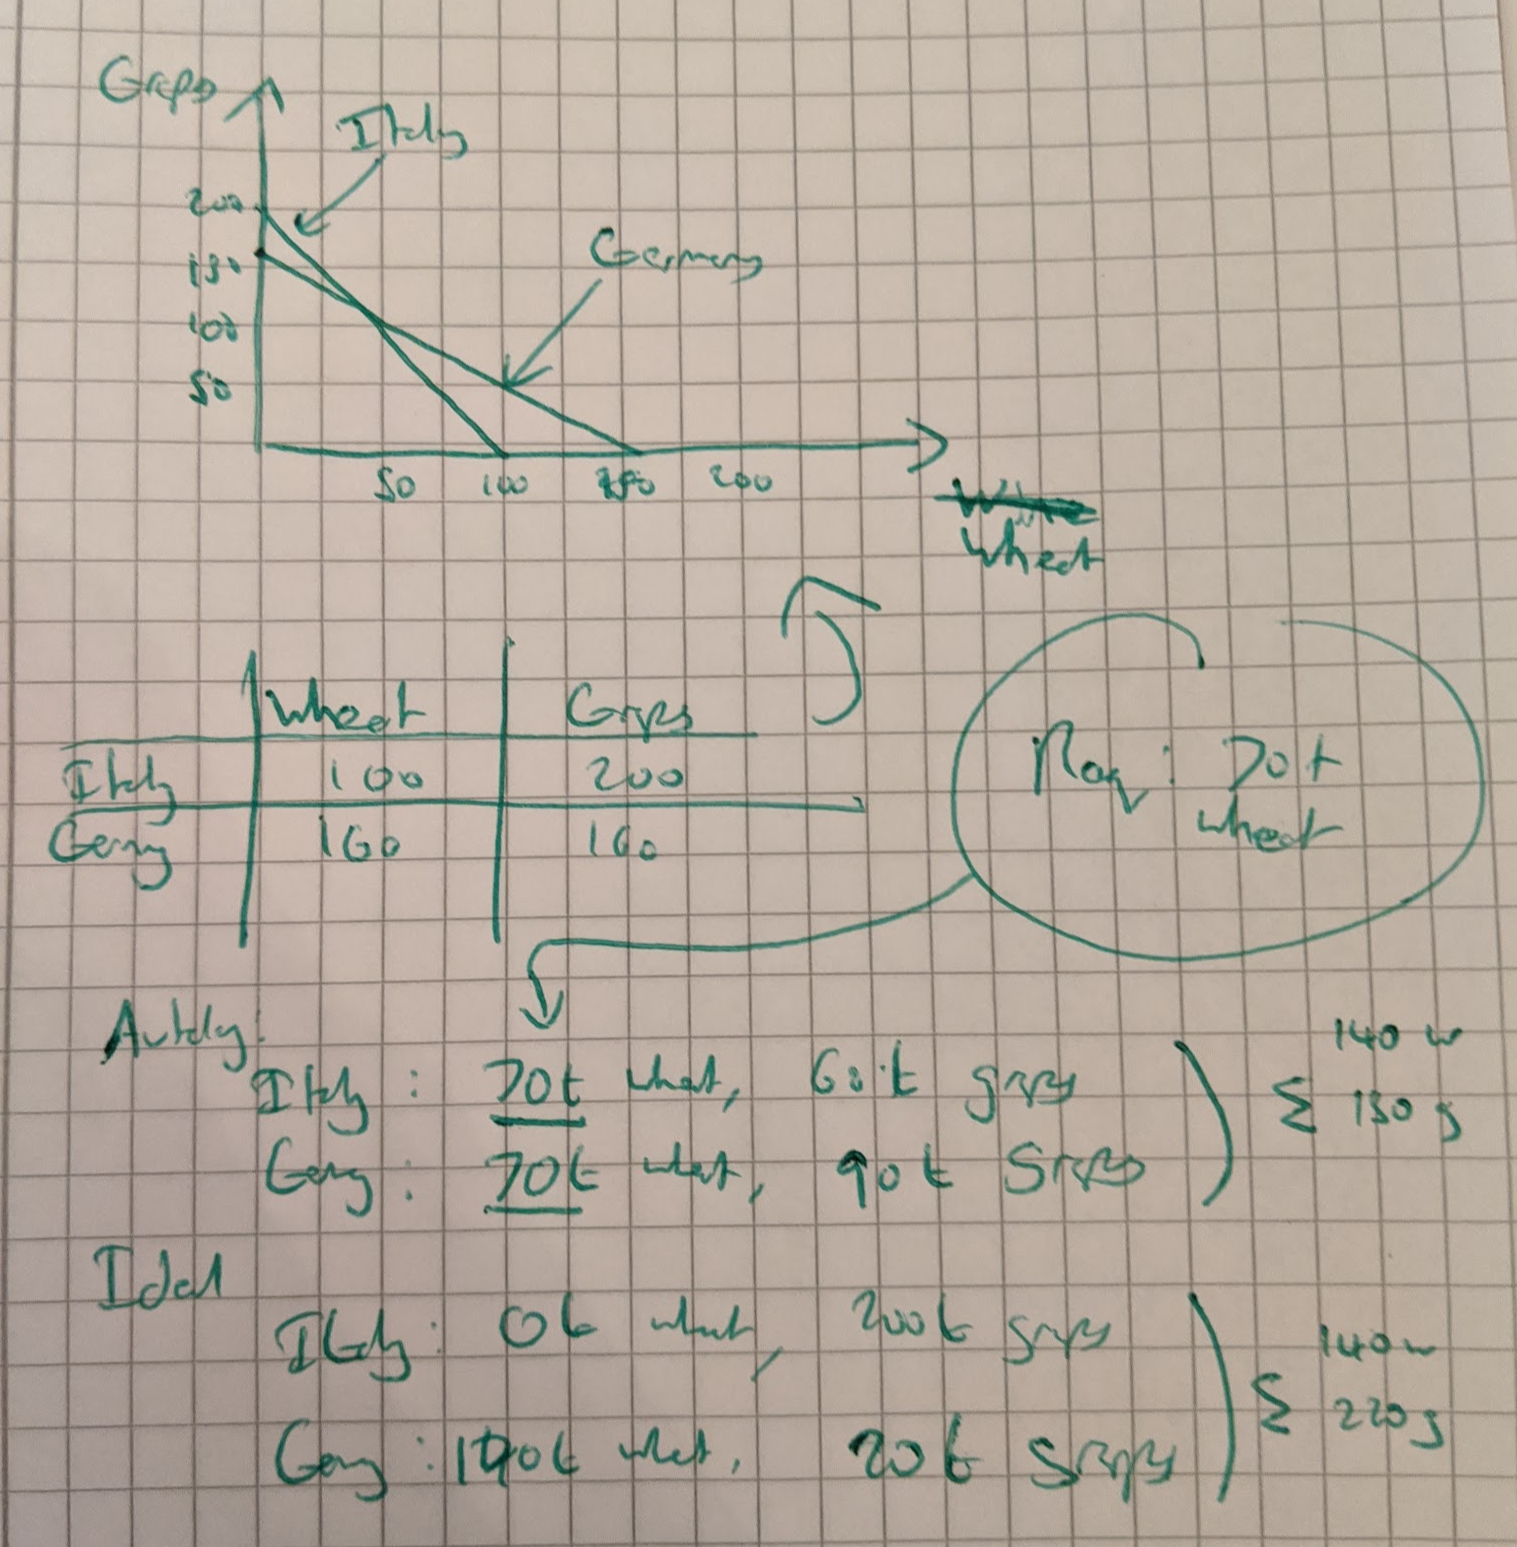
\includegraphics[width=.9\linewidth]{img/screenshots/Conflict_And_Cooperation_Beyond_The_Nation_State/2020-07-18_21-41-32_screenshot.png}
\end{center}
\item They both require 70 tonnes of wheat, and if they trade freely
(intersection on the graph), then they
will end up with more grapes overall (220t as opposed to 150t).
\item See example at the end of the section.
\item Even if one country has an advantage in both cases, we can look at the
relative cost of producing a good (here, in Germany, one tonne of wheat
costs one tonne of grapes but in Italy, one tonne of wheat costs 2 tonnes
of grapes).
\item Trade is still beneficial to both countries even when one country is
more efficient in both goods, as long as the countries differ in their
relative efficiency (so each has a comparative advantage)
\begin{itemize}
\item This is true for all countries, since there are no cloned countries
\end{itemize}
\end{itemize}
\item So, why isn't there free trade all the time?
\item Realist explanations
\begin{itemize}
\item "Security externalities" say that though trade is beneficial to both
parties, the gains from trade can let countries free up resources to do
other things. Some of these other things could be building up a military.
\begin{itemize}
\item So, countries might just want to trade with alliance partners as to avoid
strengthening potential enemies.
\end{itemize}
\item Hegemonic Stability Theory
\begin{itemize}
\item Maintaining a free trade environment might be thought of a public
good (given that domestic politics has an incentive to limit free trade)
\item Having an international system of free trade requires a hegemonic
country that is able to enforce it
\item Economic theory says that free trade should act as an equalizing force
between countries
\item This means that by enforcing free trade, the hegemon would actually
undermine itself
\end{itemize}
\item Interdependence theory
\begin{itemize}
\item A is dependent on B if the condition of A is determined or affected by B
\item Interdependence is mutual dependence (doesn't have to by symmetrical)
\item International interdependence is when countries are interdependent
\item Interdependence increase the costs of war and decreases the likelihood
of violence
\item But\ldots{} some groups are willing to sacrifice economic prosperity for
other (e.g. nationalistic) goals
\end{itemize}
\end{itemize}
\item Statist explanations
\begin{itemize}
\item National autonomy and self sufficiency can be important for countries
\item Tariffs are a source of government revenue
\begin{itemize}
\item You only indirectly take from the pockets of citizens so it's not
strongly opposed, and it's easy to implement
\end{itemize}
\item Some countries will try to protect young industries from international
competition to let them grow
\begin{itemize}
\item These industries get used to the tariff protection and lobby hard
against removal
\item Worked for Asian tigers, but they weren't democracies
\end{itemize}
\item Maximising value added in the country
\begin{itemize}
\item Lots of value added at the higher design levels, little at the raw
material production levels
\item Governments have an incentive to keep higher levels in the country
\end{itemize}
\end{itemize}
\item Economic interest explanations
\begin{itemize}
\item The Heckscher Ohlin model tries to explain why countries choose
protectionism despite there being mutual advantages for free trade:
\begin{itemize}
\item Countries have multiple resources (e.g. labour and land)
\item But differ in abundance of resources (e.g. UK has lots of labour
relative to land because it is densely populated, US is the opposite).
This is based on the ratio of resources.
\item Thus, the resources are relatively more expensive between countries
\item Produced goods require different amounts of resources to produce
\item These resources are rival between the goods produced, i.e. if you use
labour to produce good A then you can't use it for good B.
\item Thus there is an opportunity cost; if you choose to use a resource to
produce good A, then you can't use it to produce good B
\item If politically powerful factions control a scarce resource (e.g. land
in the UK, labour in the US), then you can expect protectionist
policies (since it would be relatively expensive and vulnerable to
relatively cheaper imports). Same in reverse
\end{itemize}
\item The specific factors model
\begin{itemize}
\item The same as above, but realises that as a country specializes in a
given resource (e.g. China specializing in providing labour), then
that resource becomes less and less abundant.
\item Thus there is a `concave production possibility frontier'
\item More specialization brings diminishing returns
\end{itemize}
\item Multinational production
\begin{itemize}
\item Many industries have production lines that span countries
\item One key reason why we haven't seen a reversion to protectionism has
been that business have lobbied for free trade because of this, rather
than a powerful hegemon
\end{itemize}
\item Other incentives
\begin{itemize}
\item New trade theory: each country should try to achieve an economy of
scale in something, as long as they do not overlap
\item New new trade theory: firm level differences in productivity mean that
different firms within a country want different outcomes for that
country (e.g. low productivity firm wants protectionism, high
productivity firm wants open trade)
\item Other concerns between countries e.g. banning imports of GMOs
\item Tax benefits (doing high value business in low tax environments)
\end{itemize}
\item Domestic explanations
\begin{itemize}
\item Median voter is important, and often a consumer who wants trade
\item But, elections are usually not decided on trade policy and the
electorate can be fairly easily manipulated
\item Power dynamics within countries can affect trade policy (e.g. if rural
districts are overweighted in elections (often are) then they can
benefit).
\item Partisan differences (both the left and right can be protectionist)
\item Differences between groups in their organizational capacity. E.g.
farmers have historically been well organized politically. (think
Gourevitch)
\item Bhagwati's law of constant protection: "Whenever you lower barriers
somewhere, the most intensely protectionist interests will find
another way to raise the barriers somewhere else"
\end{itemize}
\item Ideological expectations
\begin{itemize}
\item Different people have different commitments to the ideology of free trade
\item When the free trade system has failed, people often turn to more
nationalistic ideas
\end{itemize}
\end{itemize}
\item Post WW2 international (free) trade regime
\begin{itemize}
\item After WW2 ended, leaders wanted to avoid a big economic crash, so
instituted two agreements.
\item GATT was a temporary agreement to instantiate free trade
\item ITO was the organization which would take time to implement, but the US
withdrew in 1950 and it collapsed, so now we just have the GATT
\end{itemize}
\item GATT:
\begin{itemize}
\item Most favoured nation principle
\begin{itemize}
\item All exports from any other country should be treated the same as
exports from your most favoured nation (closest ally)
\item Exception for regional trade agreements
\end{itemize}
\item National treatment; foreign goods are to be treated the same as
domestic goods
\item Rules against:
\begin{itemize}
\item Dumping (selling in one country more cheaply than another)
\item Predatory pricing (below cost selling)
\item Subsidies (financing domestic companies to increase international
market share)
\end{itemize}
\item Turn quotas and other restrictions into tariffs, which are now the
main instrument of trade policy. This is 'tarrification'.
\item Multilateral trade negotiations are designed to gradually lower tariffs
\begin{itemize}
\item Idea is that both sides pick a tariff to lower
\item Tariffs are lowered for everybody by the most favoured nation principle
\item Tariffs are gradually removed
\end{itemize}
\item Dispute resolution:
\begin{itemize}
\item Dispute panel and an appellate body
\item Whoever lost had to agree to the outcome so this rarely happened
\item The WTO has a new dispute settlement mechanism that is binding, but
the Trump administration has vetoed it by not nominating a new judge
\end{itemize}
\item There are still trade barriers that are not covered
\begin{itemize}
\item Voluntary export restrictions (one country avoids exporting to another
country to avoid a protectionist backlash from it)
\item Anti-dumping measures are abused (it takes a long time to investigate
dumping, and you can put barriers up until it is complete)
\item Governments found ways to subsidize industries through regulation
\item Administrative procedures can be a barrier to trade (e.g. forcing
trade to go through lots of silly hoops)
\end{itemize}
\item Success?
\begin{itemize}
\item Trade has gone up
\item But maybe just because transport costs dropped loads
\item But tariffs did go down too
\end{itemize}
\end{itemize}
\end{itemize}
\end{itemize}
\subsection{Governing Global Markets}
\label{sec:orgeb55adb}
\subsubsection{Tim Büthe and Walter Mattli; The Rise of Private Regulation in the World Economy}
\label{sec:orgcbc1cb1}
\begin{itemize}
\item Standards between companies/countries mean accurate and comparable financial reports
\item This shapes research funding, executive compensation and many other important things
\item The US banking standard changed to the UK one in 2008 which was a big shift
\begin{itemize}
\item From a litigation based system to a principles based one
\end{itemize}
\item Other countries followed suit, now 120 countries use it (2010)
\item International integration of financial markets and more multinational
companies created that shift
\begin{itemize}
\item Divergence has costs too, often higher than (one time costs of) switching systems
\end{itemize}
\item Governments privatize regulation because they lack the necessary technical
expertise, resources or the flexibility to deal with urgent cases
\item National standards have been declining as international standards have been increasing
\item Why?
\begin{itemize}
\item The WTO obliges the use of international standard unless they are
inappropriate or ineffective
\item Standards define best practices and help reduce legal liability
\item Standardized trade reduces transaction costs. Bringing standards to
unstandardized trade would reduce transaction costs equivalent to removing
several percent worth of tariffs
\item This benefits firms (lower overheads) and consumers (more access to products)
\end{itemize}
\item Standard setting organizations like the ISO and IEC are private organizations
\item Understanding who holds power in these organizations is important
\item International standards say that science is the same everywhere, but this is
naiive. There is often no right or wrong answer for standards, but many
details that are important for countries.
\item Countries have huge interests in setting good standards
\item International standards organizations rely on national level standards
organizations, but these differ in their capacities
\item Countries with strong, single and unified national standard setting bodies
often have lots of success when influencing international standards (US),
countries with many competing national bodies have less success (EU).
\end{itemize}
\subsubsection{Tim Bartley; Certifying Forests and Factories:  States, Social Movements, and the Rise of Private Regulation in the Apparel and Forest Products Field}
\label{sec:org062db30}
\begin{itemize}
\item Private regulation has emerged to address some environmental and labour issues
\item The following was important for that to occur:
\begin{itemize}
\item Social movement campaigns that targeted companies
\item Neo-liberal institutional context for business
\end{itemize}
\item Standards have gone from a top down national model to a bottom up market
mechanism model
\item Private regulation organizations:
\begin{itemize}
\item Forest Stewardship Council, Sustainable Forestry Initative and CSA-International
\item Fair labor association ,social accountability international, worldwide
responsible apparel production
\end{itemize}
\item These organizations were not planned, but sprung up from coalitions and nonprofits
\item Both industries ended up at the same solution.
\item Potential problems with regulation:
\begin{itemize}
\item Greenwashing (changing an image without changing practices)
\item Private regulation conflicts with openness and accountability
\item Private regulators have little power to enforce anything in contrast to
public regulators
\end{itemize}
\item General findings of a common cause for the two industries:
\begin{itemize}
\item Social movements and neoliberal (low regulation) context
\item NGOs were repeatedly defeated in international trade negotiations, so they
tried a different approach (of private regulation)
\item Free trade limited direct state action (e.g. Austria was accused of
violating the GATT by preventing imports of unsustainable timber)
\item Social movement pressure:
\begin{itemize}
\item Public attention peaked in the \textasciitilde{}early 90's, and pressure made the
unsustainable companies form buyers groups, which created a demand for
sustainable timber and good labor conditions
\end{itemize}
\item States supported private regulation
\begin{itemize}
\item Free trade rules limited direct government action
\item States then funded private regulators themselves
\item But poorer countries that were exporting were opposed to regulations
(Global North-South conflict).
\end{itemize}
\end{itemize}
\end{itemize}
\subsubsection{Tim Büthe and Walter Mattli; Implications for Global Governance}
\label{sec:orgd0a6f44}
\begin{itemize}
\item Regulation is increasingly privatized, and the representation of national
interests is increasingly done via private domestic regulators
\item Some systems have one domestic regulator, while others have many. Many domestic
regulators (EU) are worse for influencing international regulation than one
domestic regulator (US).
\item Implications for public policy:
\begin{itemize}
\item Institutional reform to improve the fit between domestic and international
regulators
\begin{itemize}
\item Firms pay a real cost for misalignment here
\item You can either:
\begin{itemize}
\item Change the existing international organization which is really hard,
because it's unlikely that a majority will agree with you
\item Create a new competing international organization with decision making
procedures that are better for you (hard too because you have to compete
with the incumbent on a global scale)
\item Change domestic institutions to make them more complimentary with the
existing international regime (this is the only realistic option).
\end{itemize}
\end{itemize}
\end{itemize}
\item Private sector regulation can promote industry interests over public interests
\item The EU has a large private sector regulator which is able to have oversight
of and give public control over private regulation
\item A similar model needs to be rolled out internationally; consumer participation
in standard setting has been dropping, and consumer representatives are often
ignored in favour of industry interests. An EU-style body is often required to
ensure public interests are maintained.
\end{itemize}
\subsubsection{James Vincent; Can Standards and Regulations Keep Up with Health Technology?}
\label{sec:org1c3711f}
\begin{itemize}
\item Technology is changing fast and making health technology change fast too, but
the regulatory structure struggles to keep up
\item Regulation is used to guide the design of new medical equipment
\item Novel technologies usually don't fit into the standards because they are novel
\item Regulatory challenges:
\begin{itemize}
\item Open source designs might be used very few times, so there is a high
regulatory burden
\item Designers might want to iterate rapidly on new tech, or test in real-life cases
\item The context that people use devices in varies lots (especially for home use,
e.g. T1 diabetes)
\begin{itemize}
\item Having more configuration of the same product can help with this, but the
development burden is increased
\item One solution is post-market analysis e.g. diaries
\end{itemize}
\item Open source or private solutions might be low quality (e.g. mobile phone
apps with bad programming).
\begin{itemize}
\item One solution is to have guidelines that developers must sick to
\end{itemize}
\end{itemize}
\item Opportunities:
\begin{itemize}
\item Ideas can be shared with new technologies like open source
\item Users can understand the constraints of a solution if they have a good
knowledge of how it works and can contact the developers
\end{itemize}
\end{itemize}
\subsubsection{Lecture}
\label{sec:org3a7266f}
\begin{itemize}
\item Product standards are important for design, sizing, performance,
interoperability, etc
\item Mass production is inconceivable without standards
\item Public interest is furthered by standards in consumer protection, workplace
safety and environmental externalities
\item Cross national differences in standards create barriers to trade (equal to
2-10\% tariffs)
\item International harmonization of standards through regulatory cooperation,
delegation of standard setting to transnational bodies is efficient.
\item Private bodies exist: ISO (International Standards Organization) and IEC
(International Electrotechnical Commission)
\begin{itemize}
\item These are non-governmental
\item One member body per country
\item Really big, 50k+ experts involved
\item Standards development is controlled by a central secretariat
\item The central secretariat and coordination between the ISO and IEC guarantees
that there is one definitive standard for a given product
\item Bottom up agenda, with adoption of standards by a super-majority
\item These are powerful bodies, and as such, whoever gets to write the actual
standards has a lot of power
\begin{itemize}
\item Countries have distributional conflicts based on business interests
\end{itemize}
\end{itemize}
\item These are the different types of standards organizations:
\begin{itemize}
\item Institutional setting for the rule making:
\begin{itemize}
\item Public
\begin{itemize}
\item Unitary (non-market based): Rule making in a focal international organization
\item Plural (market based selection): Competing standards developed by
national/regional bodies
\end{itemize}
\item Private
\begin{itemize}
\item Unitary: Transnational focal institution
\item Plural: Competing standards from individual firms (e.g. Microsoft or
consortia)
\end{itemize}
\end{itemize}
\end{itemize}
\item Institutional complementarity theory
\begin{itemize}
\item International standardization has adjustment costs and thus distributional
conflicts
\item Institutional complementarity (see Buthe/Mattli above) is the functional fit
between the domestic institutions and the international level.
\begin{itemize}
\item This affects the ability of domestic players to influence international standards
\end{itemize}
\end{itemize}
\item Key elements of the ISO and IEC process:
\begin{itemize}
\item They are the focal points of international standard setting
\item There is a multi-stage rule making procedure which tries to settle the
fundamentals early on, and then increases the specificity of the drafts as
time goes on
\item The preferences of everybody are tried to be understood and integrated to
get a consensus
\item Countries with a greater institutional capacity can better influence the stages
\begin{itemize}
\item They need expertise, material resources, information about the
international standardization politics, and the ability to know what is in
their interest on a domestic level (domestic preference aggregation)
\item Hierarchical systems are good at this (US good, UK bad)
\end{itemize}
\end{itemize}
\end{itemize}
\subsection{The Politics of Economic Development}
\label{sec:org12accd4}
\subsubsection{Tim Büthe, Solomon Major, and André de Mello e Souza; The Politics of Private Foreign Aid: Humanitarian Principles, Economic Development Objectives, and Organizational Interests in the Allocation of Private Aid by NGOs.}
\label{sec:org8bc2ab8}
\begin{itemize}
\item Lots of foreign aid is raised from non-governmental sources, but up until
recently (this paper) we didn't know how it was distributed.
\item Private donations make up 60\% of aid, and private money makes more and more
decisions of what gets funded in poor countries
\item There is lots of literature on public aid, but little on private aid
\item A common identity shapes NGO interactions around a "principled issue network"
which shapes members around their values rather than material concerns
\item There are two types of altriusm here for NGOs which explain private aid:
\begin{description}
\item[{Humanitarian discourse}] Find underdeveloped or neglected populations and
provide them with services
\begin{itemize}
\item People should get aid based on objective need
\item Oriented around an ethical obligation to relieve suffering
\item Tries to be impartial, neutral and independent
\item Prioritizes by need and distress, ignores race, gender etc
\item Wide acceptance
\end{itemize}
\item[{Development discourse}] Focus on root causes of poverty and aim for
sustainable improvements in the long term
\begin{itemize}
\item People should get aid based on whether it can contribute to sustained
development
\item Concerned with outcomes rather than intentions
\item Aims for persistent increases in socioeconomic, political or physical
well being
\item The better suited the recipient's environment is to development aid, the
more that objective need plays a role in determining aid allocation
\end{itemize}
\end{description}
\item A third explanation for private aid is:
\begin{description}
\item[{Fundraising discourse}] NGOs allocate funds to opportunities that can
increase fundraising capacity based on what is currently in the media
\begin{itemize}
\item Cynics are skeptical of NGOs good intentions
\item NGOs can fail organizationally or systemically, e.g. if they want to grow
bigger or self perpetuate, they might act in their own interests.
\item NGOs can be seen to operate in a competitive market for aid funding and
aid delivery.
\item NGOs sometimes need to be present for world events so that they can show
their presence to donors
\end{itemize}
\end{description}
\item Public donors use discretion to allocate aid that serves their own interests
\item NGOs act more like a group and are mutually respecting and supporting, which
supports their group discourses
\item Conclusion / empirical findings:
\begin{itemize}
\item Humanitarian discourse is strongly supported
\item Development discourse is weakly supported
\item No support for fundraising discourse
\item Low salaries and unpleasant conditions mean that the NGO industry is
self-selecting for those who want to do good work.
\end{itemize}
\end{itemize}
\subsubsection{Lecture}
\label{sec:org9f5d1d9}
\begin{itemize}
\item Economic growth is the following:
\begin{itemize}
\item GDP = C + I + G
\begin{itemize}
\item Consumer spending
\item Investment
\item Government spending
\end{itemize}
\end{itemize}
\item Economic growth is varied by the institutional context in which it occurs
\item[{Institutions}] Stable, valued and recurring patterns of order like schools
\item Three institutions are important for economic growth:
\begin{itemize}
\item Property rights
\item Rule of law
\item Independent courts
\end{itemize}
\item[{Resource curse}] When natural resource wealth allows the state to access
wealth without having to tax citizens, which means citizens lose a level over
which it can control government (willingness to pay tax), so the government
doesn't develop properly and performs poorly
\item Types of foreign aid:
\begin{itemize}
\item Military aid
\item Humanitarian/emergency/development aid
\item Teaching assistance/state building/administrative training
\end{itemize}
\item Distinctions of aid:
\begin{itemize}
\item Direct vs indirect (e.g. country to country or via the world bank/EU/etc)
\item Different mechanisms of delivery (goods, cash, etc)
\item Grants vs loans
\item Official government aid or private aid
\item OECD says official aid is:
\begin{itemize}
\item Administered to promote economic development and welfare of the recipient
as the main objective, with at least 25\% grants
\end{itemize}
\end{itemize}
\item Countries give aid because:
\begin{itemize}
\item Physical security for the donor (avoid spillover conflicts)
\item Increase the donor's political influence (e.g. reward 'good' UN voting histories)
\item Donor's economic self-interest (developing markets abroad)
\item Try to maintain global peace, disease eradication etc (protect the global commons)
\item Increase the donor's reputation
\item Out of a sense of duty or altruism
\end{itemize}
\item Why not to give aid:
\begin{itemize}
\item There is a moral hazard because the recipient could chose to not develop
because it is guaranteed aid
\item Aid dependency trap (economy never develops because aid is given, local
markets cannot compete with aid and die)
\item Donor's economic self interest (might be a hidden subsidy for domestic firms)
\item Donor's reputation (might be artificially raised)
\item It might not be a good use of money compared to other things
\end{itemize}
\item The OECD decided in 1970 to donate 0.7\% of GDP for foreign aid.
\begin{itemize}
\item Few countries make this (about 5)
\item US gives about 0.16\%; congress never supported 0.7\%, only the executive
\end{itemize}
\item Drivers of aid:
\begin{itemize}
\item Alliance partners (same reasons as why countries trade with alliance
partners)
\item Geopolitical strategic importance (Somalia got loads of aid until the cold
war ended, then it stopped and the country collapsed)
\item UN voting record
\item UN Security Council seat (brings lots more aid when a country receives it)
\item Trade (export opportunities for the donor)
\item Good governance in the recipient country (so the money isn't wasted)
\item Recipient need (but this is inconsistent)
\end{itemize}
\item Private aid
\begin{itemize}
\item Private sources are agenda setters
\item Sources include:
\begin{itemize}
\item Business charitable giving (financial, managerial, volunteer time, etc)
\item Individuals donations
\item Foundations
\begin{itemize}
\item Old ones: Rockefeller, Ford, etc
\item New ones: Gates
\item Fast growing sector
\item Lots of agenda setting power
\end{itemize}
\item Private sources aggregate funds from many countries and spend them together
\item The allocation decision is not influenced by governments
\end{itemize}
\end{itemize}
\end{itemize}
\section{Political Science and Public Policy}
\label{sec:org8cc47d9}
\subsection{Jake Bowers and Paul Testa; Better Government, Better Science: The Promise of and Challenges Facing the Evidence-Informed Policy Movement}
\label{sec:org2165de7}
\begin{itemize}
\item Evidence can be used for evaluation (what worked) or insight (why did it work)
\item What does evidence mean, and what is evidence based policy?
\begin{itemize}
\item Evidence can be peer reviewed studies or future studies that assess the
success of policy interventions
\item Policies should be judged that shares the authority of science, i.e. it
should be impersonal, transparent and unbiased
\item Policy can be "evidence informed" as opposed to "evidence based" when social
scientists advise rather than set policy
\end{itemize}
\item Organizations can use experiments and randomized trials to determine whether a
policy worked. Randomized trials are especially good because they can be
easily compared.
\item An example is having defaults:
\begin{itemize}
\item E.g. default organ donation
\item They are low-touch and don't require lots of intervention
\item They lower the transaction costs for most people
\item Defaults are implicitly endorsed by experts, which is good for people who
lack expertise
\end{itemize}
\item Problems:
\begin{itemize}
\item Sometimes evidence based policies are seen as paternal
\item They can be seen as the government intervening in the lives of citizens
\item The policymaker might be more of a salesperson than an objective evaluator
\item There is nothing to say that academics will actually create good policies;
perhaps their analysis is still wrong or they lack the right tools
\item Results from studies might not generalize into the proposed use case
\begin{itemize}
\item Having multiple teams around the world working on parallel identical
studies can help
\end{itemize}
\item If trials only show what works, then we might not tell us anything about
new phenomena
\begin{itemize}
\item E.g. in Tennessee, a trial showed that small classes in schools produce
better outcomes, but in California the policy was implemented by using
more new teachers which led to worse outcomes
\item It is important to try to understand the 'why' behind studies
\end{itemize}
\item Scholars might try to oversell results
\item Scholars might not publish null results, but these are still useful for
finding out what doesn't work
\end{itemize}
\end{itemize}
\subsection{Helen Milner and Sondre Ulvund Solstad; Technology Diffusion and the International System}
\label{sec:org97c20ad}
\begin{itemize}
\item States rely on technology being invented abroad, and technology development
affects economic development
\begin{itemize}
\item States mostly import technologies rather than creating their own
\item Adoption of technology is costly and disruptive
\item Thus most new technologies are resisted by interest groups \& governments
\item Government policies are critical to slowing down or speeding up technology development
\end{itemize}
\item \href{Cardwell's Law.org}{Cardwell's law}: No nation has been very creative for more than an historically
short period. Fortunately, as each leader has flagged there has always been,
up to now, a nation or nations to take up the torch."
\item During 'long waves', technology diffused quickly through the international
system and at other times it was slow
\item Internal state politics:
\begin{itemize}
\item Governments want support from consumers and firms and want to perpetuate the state
\item Firms want the government to not support new technology, but provide
national defense
\item Consumers want national defense, but also new technology under the
assumption that it will increase their welfare
\end{itemize}
\item This paper argues that:
\begin{itemize}
\item The external pressures of states to innovate changes over time
\begin{itemize}
\item When threats from abroad are greater than threats to the government from
domestic forces with vested interests in existing technology, then
governments will encourage technology adoption
\item If there is lots of competition in the international system, there is more
pressure to adopt new technologies
\end{itemize}
\item Systemic pressures are related to the distribution of capabilities in the
international system
\begin{itemize}
\item The benefits of a technological leader are great, and allow states to
coerce other states
\item There is an inverse correlation between violent international competition
and system concentration (more equally sized states means more competition)
\item Neighborhood threats are positively related to technology adoption
\item Civil war is negatively related to technology adoption
\item Further away inventions take longer to adopt
\item Less concentration leads competitive pressures and more tech innovation
\end{itemize}
\item Systemic shifts can be linked to global technology waves
\end{itemize}
\item Example: Swiss government establishing railroads
\begin{itemize}
\item Railroads hadn't been passed in the Swedish parliament for 25 years
\item Then once the Crimean war broke out they were passed in weeks
\item At some points after this, Sweden spent 15\% of expenditure on railroads
\item Their setup was inefficient, with a main line inland, and branches to
settlements on the sea intended to make Sweeden more defensive.
\end{itemize}
\end{itemize}

\subsection{Lecture}
\label{sec:org9f11c85}
\begin{itemize}
\item Science gives us another way of knowing things; in particular we can say "it
never happened but we know that it is true"
\item It lets us cope with and systematically reduce uncertainty in life
\item Unlike physical sciences, social science has the following difficulties:
\begin{itemize}
\item Few observations but many variables
\item Little chance for genuine experimentation
\item Findings seem intuitive after you find them
\begin{itemize}
\item Common sense is a grab bag of logically inconsistent beliefs that can work in
specific contexts, but don't work well when generalized because they lose all
the context from the specific situation.
\end{itemize}
\item High complexity (linked to the first one)
\end{itemize}
\end{itemize}
\end{document}
